\documentclass[11pt]{beamer}
\usepackage[utf8]{inputenc}
\usepackage[T1]{fontenc}
\usepackage{lmodern}
\usepackage[spanish, es-tabla]{babel}
\usepackage{graphicx}
\usetheme{Berlin}
\usepackage{listings}
\usepackage{tikz}
\usepackage{pgfplots, pgfplotstable}
\usepgfplotslibrary{statistics}

\renewcommand{\lstlistingname}{Codigo}
\renewcommand{\lstlistlistingname}{Lista de \lstlistingname s}

\setbeamertemplate{date}{}

\begin{document}
	\author{Luis Augusto Sandoval \and Gerardo Diaz}
	\title{Presentación de funcionamiento y despliegue}
	%\subtitle{}
	%\logo{}
	%\institute{}
	%\subject{}
	%\setbeamercovered{transparent}
	%\setbeamertemplate{navigation symbols}{}
	\begin{frame}[plain]
		\maketitle
	\end{frame}
	
	\begin{frame}
		\frametitle{Diagrama resumen del funcionamiento de una cache asociativa por conjuntos de 4 vias}
		\begin{figure}
			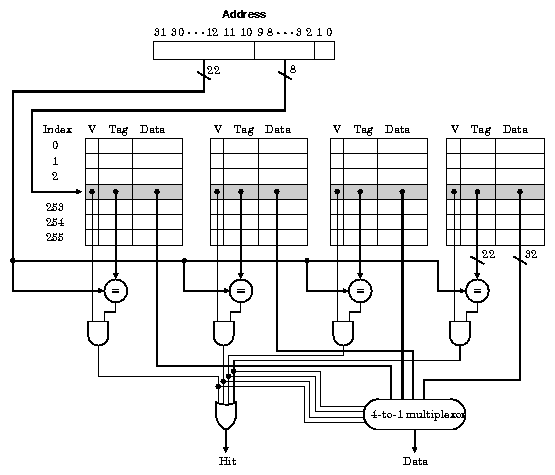
\includegraphics[width=0.6\textwidth]{setAssociative.png}
		\end{figure}
	\end{frame}
	
	\begin{frame}
		\frametitle{Resumen de las clases}
		\begin{itemize}
			\item \textbf{CacheRequest}: Simula las consultas a cache por parte del CPU
			\item \textbf{CacheLine}: Simula las lineas de la cache. Bloques en correspondencia directa o conjuntos en asociativa por conjuntos.
			\item \textbf{PrefetchBuffer}: Simula un buffer de prefetching de adyacencias. Guarda en memoria el bloque siguiente y el anterior a la dirección previa consultada.
			\item \textbf{SetAssociativeCache}: Clase contenedora con la lógica para hacer funcionar las clases anterior y simular el funcionamiento de una memoria cache en conjunto
		\end{itemize}
	\end{frame}
	
	\begin{frame}
		\frametitle{Funcionamiento del prefetching}
		
		\begin{equation}
			bloqueSiguiente = D + (W * B * 8)
		\end{equation}
		\begin{equation}
			bloqueAnterior = D - (W * B * 8)
		\end{equation}
		
		\begin{itemize}
			\item \textbf{D} es la dirección, \textbf{W} el tamaño de la palabra en bytes y \textbf{B} el tamaño del bloque en palabras.
			\item \textbf{D} en \textbf{bloqueSiguiente} no puede ser mayor a la dirección máxima de la cache ni \textbf{D} en \textbf{bloqueAnterior} menor a 0
			\item Si alguna de las 2 condiciones no se cumple, entonces no se tomara el bloque correspondiente
		\end{itemize}
	\end{frame}
	
	\begin{frame}
		\frametitle{Benchmark}
		\begin{itemize}
			\item \textbf{Execution time}: El tiempo de ejecución real del programa. Se dice tiempo real porque descarta el tiempo tomado por el sistema operativo y el kernel.
			
			\item \textbf{CPU usage}: El tiempo que el sistema Operativo destina a la ejecución del programa, es decir, el tiempo destinado al programa menos el tiempo de CPU que el S.O. destino a la ejecución de otros programas durante la ejecución.
			
			\item  \textbf{RAM usage}: El uso total de RAM por el programa.
		\end{itemize}
	\end{frame}
	
	\begin{frame}
		\frametitle{IaC y Terraforming}
		Para simular el entorno del laboratorio se utilizaron herramientas como Docker y se omitió el uso de librerías externas o no estándares.
		
		La imagen de Docker destinada a la ejecución del programa utiliza como base Ubuntu 14.04, la cual trae consigo Python 3.4.3.
		
		Se evito el uso de librerías no estándares y de módulos o librerías externas.
	\end{frame}

	\begin{frame}
		\frametitle{Generación de Direcciones}
		\begin{figure}[h]
			\centering
			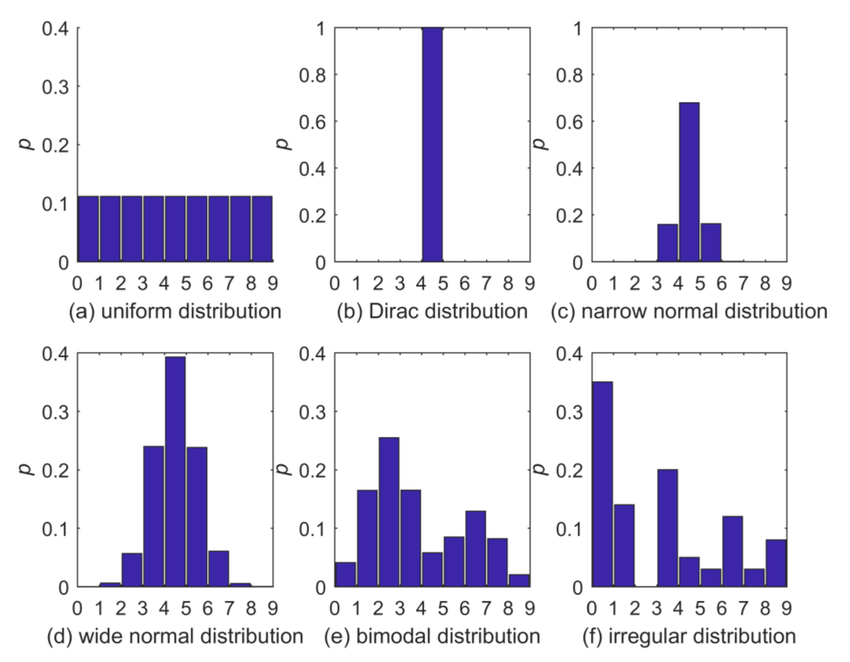
\includegraphics[width=0.65\textwidth]{test_distributions.png}
			\caption{Tipos de Distribuciones Estándar}
			\label{fig:uni_normal_dist}
		\end{figure}
	\end{frame}

	\begin{frame}
		\frametitle{Generación de Direcciones}
		\begin{figure}[ht]
			\centering
			\begin{minipage}[t]{0.48\textwidth}
				\centering
				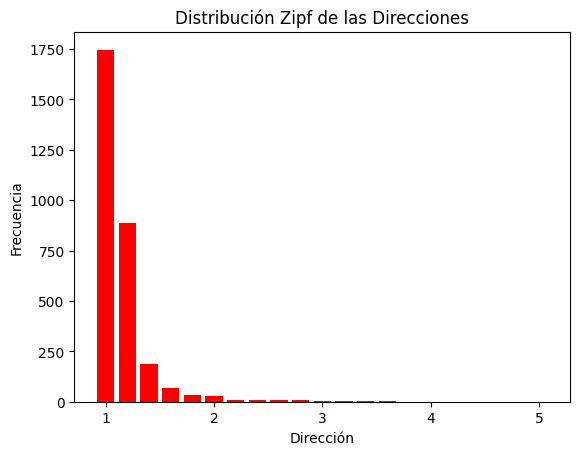
\includegraphics[width=\textwidth]{zipf.png}
				\label{fig:zipf_dist}
			\end{minipage}
			\begin{minipage}[t]{0.48\textwidth}
				\centering
				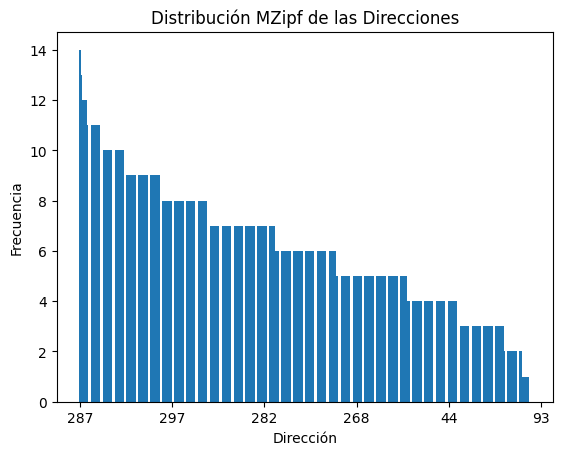
\includegraphics[width=\textwidth]{mzipf.png}
				\label{fig:mzipf_dist}
			\end{minipage}
			\caption{Distribución Zipf y Modified-Zipf con datos del simulador}
		\end{figure}
	\end{frame}

	\begin{frame}
		\frametitle{Eficacia del Simulador}
		\begin{tikzpicture}
			\begin{axis}
				[
				width = {0.68\textwidth},
				title = {Comparación entre Distribuciones},
				xlabel = {Número de Accesos},
				ylabel = {Tasa de Aciertos (\%)},
				xtick distance = {1000},
				ytick distance = {10},
				legend pos = {outer north east},
				legend cell align = {left}
				]
				\addplot[only marks, color=red, restrict x to domain=0:3000]
				table[x=AccessCounter,y=HitRate,col sep=comma] {zipf.csv};
				\addlegendentry{Zipf}
				
				\addplot[only marks, color=blue, restrict x to domain=0:3000]
				table[x=AccessCounter,y=HitRate,col sep=comma] {mzipf.csv};
				\addlegendentry{MZipf}
				
				\addplot[only marks, color=teal, restrict x to domain=0:3000]
				table[x=AccessCounter,y=HitRate,col sep=comma] {normal.csv};
				\addlegendentry{Normal}
				
				\addplot[only marks, color=purple, restrict x to domain=0:3000]
				table[x=AccessCounter,y=HitRate,col sep=comma] {augustus.csv};
				\addlegendentry{Augustus}
				
				\addplot[only marks, color=orange, restrict x to domain=0:3000]
				table[x=AccessCounter,y=HitRate,col sep=comma] {uniform2^16.csv};
				\addlegendentry{Uniforme $2^{16}$}
				
				\addplot[only marks, color=yellow, restrict x to domain=0:3000]
				table[x=AccessCounter,y=HitRate,col sep=comma] {uniform2^32.csv};
				\addlegendentry{Uniforme $2^{32}$}
			\end{axis}
		\end{tikzpicture}
	\end{frame}
	
	\begin{frame}
		\frametitle{Eficiencia del Simulador}
			\begin{table}[ht]
				\centering
				\resizebox{\linewidth}{!}{%
				\begin{tabular}{|c|c|c|c|}
					\hline
					\multicolumn{4}{|c|}{CPU de 4 núcleos y 3,90 \textit{Ghz} de frecuencia} \\
					\hline
					\textbf{Método de Generación} & \textbf{Tiempo de Ejecución (\textit{s})} & \textbf{Uso de CPU (\%)} & \textbf{Uso de RAM (\textit{MB})} \\
					\hline
					Augustus 			& 16.70  & 5.51 & 26.87 \\
					Uniforme $2^{32}$	& 14.88  & 4.84 & 26.82 \\
					Uniforme $2^{16}$	& 14.05  & 4.84 & 25.84 \\
					Normal 				& 17.01  & 5.64 & 25.97 \\
					Zipf   				& 250.92 & 0.28 & 25.89 \\
					MZipf  				& 16.80  & 5.60 & 25.50 \\
					\hline
					\multicolumn{4}{|c|}{CPU de 2 núcleos y 3,20 \textit{Ghz} de frecuencia} \\
					\hline
					\textbf{Método de Generación} & \textbf{Tiempo de Ejecución (\textit{s})} & \textbf{Uso de CPU (\%)} & \textbf{Uso de RAM (\textit{MB})} \\
					\hline
					Augustus 			& 25.66	 & 4.21 & 26.57 \\
					Uniforme $2^{32}$ 	& 25.07	 & 4.79 & 26.64 \\
					Uniforme $2^{16}$ 	& 25.37	 & 4.73 & 25.41 \\
					Normal 				& 25.68	 & 4.52 & 25.85 \\
					Zipf   				& 450.06 & 0.40 & 26.19 \\
					MZipf  				& 27.03	 & 4.85 & 25.28 \\
					\hline
				\end{tabular}}
				\caption{Resultados del \textit{benchmark}}
			\end{table}
	\end{frame}
	
\end{document}